%\begin{tikzpicture}
%\matrix (root)  [table, text width=7mm, name=root]
%{ 30 & {} & {} & {} & {} \\};
%\matrix (lvl1c) [table, text width=7mm, name=lvl1c, below of=root]
%{ 33 & {} & {} & {} & {} \\};
%\matrix (lvl1l) [table, text width=7mm, name=lvl1l, left of=lvl1c]
%{ 24 & {} & {} & {} & {} \\};
%\matrix (lvl2r) [table, text width=7mm, name=lvl1r, right of=lvl1c]
%{ 17 & {} & {} & {} & {} \\};
%\matrix (tape)  [table, text width=7mm, name=new, below of=lvl1r]
%{ 30 & {} & {} & {} & {} \\};
%\end{tikzpicture}

\begin{figure}
	\centering
%	\includegraphics[width=\textwidth]{topic/sampletrie_drawn}	
	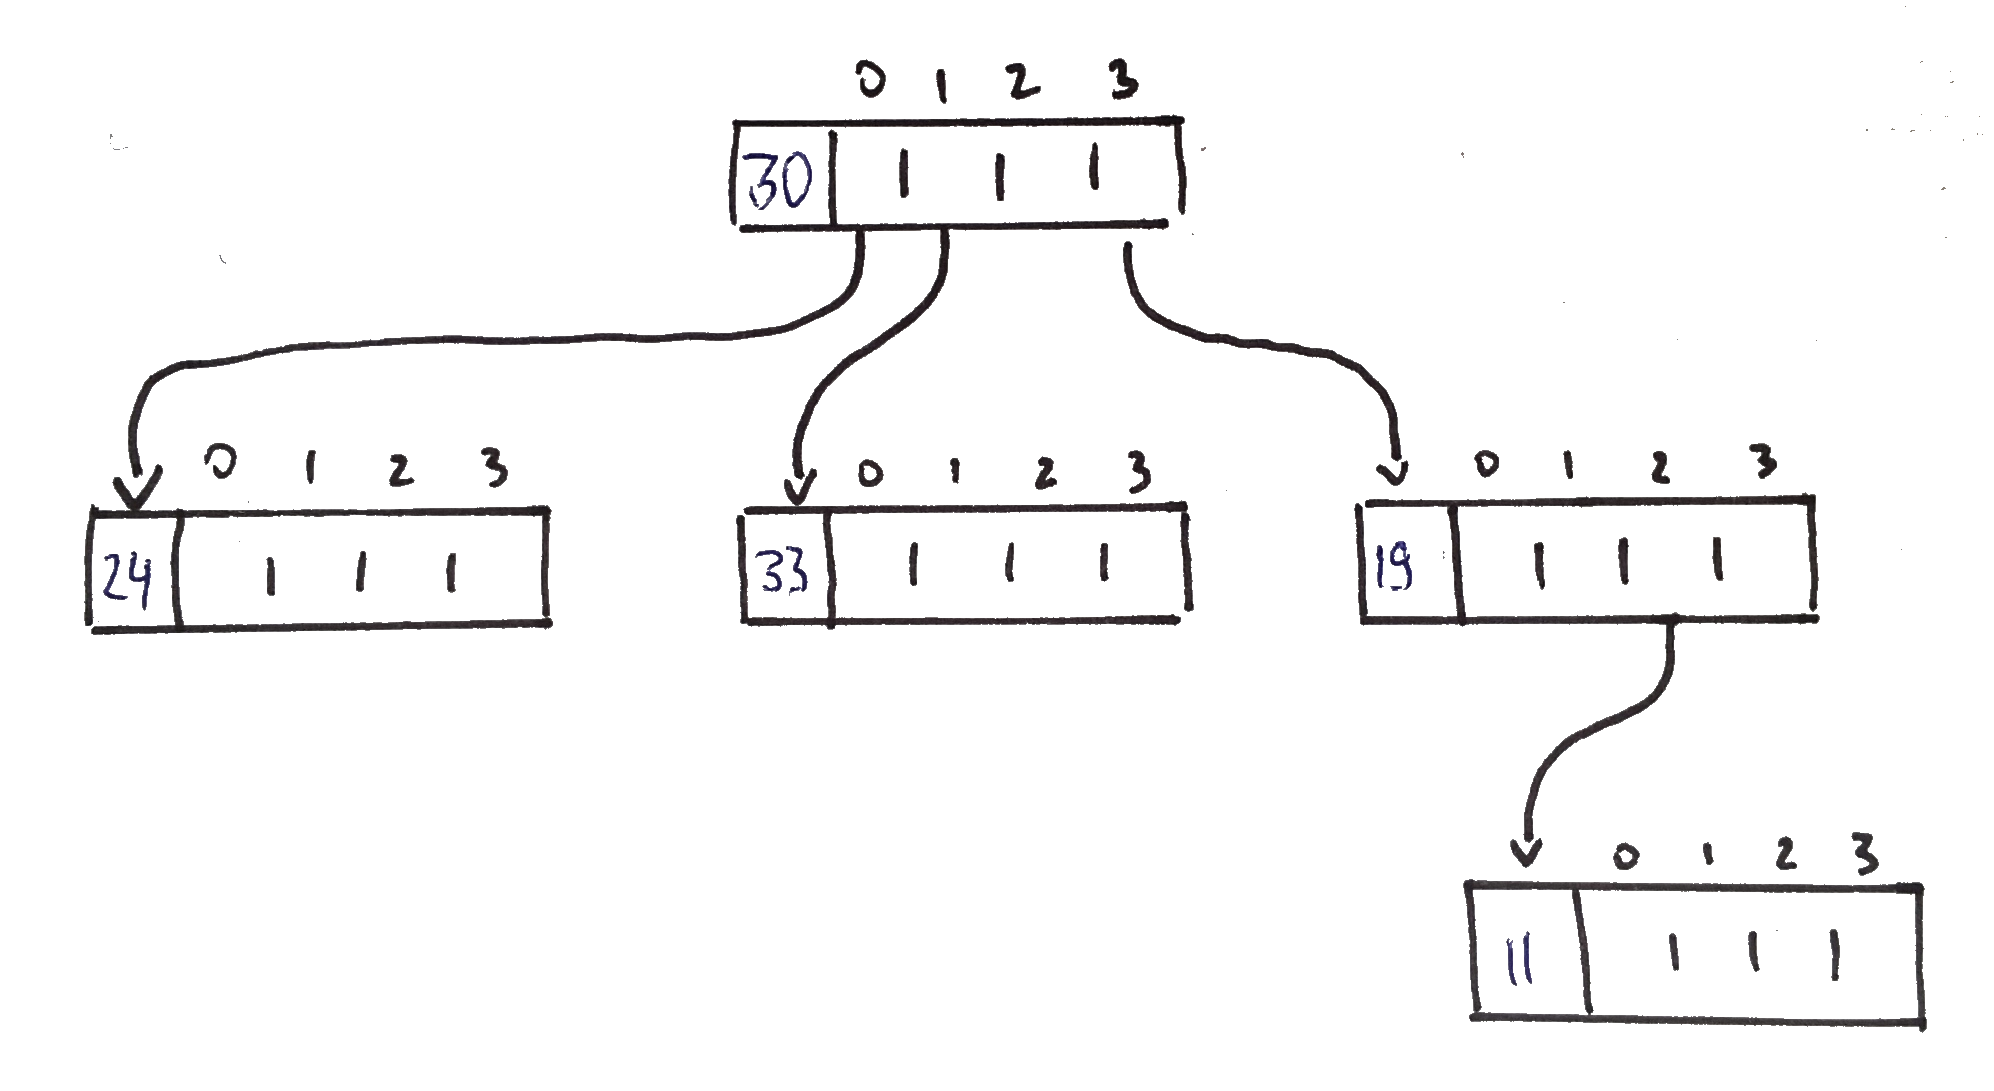
\includegraphics[width=\textwidth]{topic/imgtries/sampletrie_drawn_transp}
	\caption{ \small A trie with $k = 4$ and entries 30, 24, 33 and 19.
		To insert 11, we repeatedly divide 11 by 4, giving
			$11 \overset{3}{\longrightarrow} 2  \overset{2}{\longrightarrow} 0$.
		The remainders 3 and 2 lead to the center right node where we insert a new node with value 11 as shown.}
\end{figure}


A trie \cite{knuth:tries} is a data structure.
In fact, a trie is a tree with the same maximum branching factor $k$ for all nodes.
A trie differs from balanced binary trees or other types of trees in the way that elements are inserted, looked up and deleted.
Every node of a trie contains an integer and $k$ pointers to its child nodes, indexed from 0 through $k - 1$.
Typically, $k$ is a power of 2.
The pointers in every node are \emph{null} initially and may be set when new elements are added.
The first element that is added to an empty trie is stored in the root and no new nodes are created.
Subsequent elements are added as follows:
Given a new element $e$, we repeatedly divide $e$ by $k$.
This gives a sequence of quotients and remainders.
Since the remainders are in the range 0 through $k - 1$, they specify a sequence of pointers.
The sequence starts at the root and descends one level into the tree with every step.
We follow the sequence of pointers until we reach a null pointer, which is where we insert a new node with value $e$.
This completes the insertion of a value into a trie.
Searching a value $v$ in a trie happens in a similar way:
First, we check for $v$ in the root.
If $v$ is not present there, we follow the sequence of remainders as above.
At every node, we check if it contains $v$.
If we eventually reach a null pointer the trie does not contain $v$, otherwise it does.
To delete a value $u$, we first search for $u$ in the trie and store the node $n_u$ which contains $u$.
Now, we locate any leaf that is a descendant of $n_u$, replace the value in $n_u$ by the leaf's value and then remove the leaf from the trie.
